
\documentclass[aps,letterpaper,10pt]{revtex4}

\usepackage{amsmath}
\usepackage{algorithmic}
\usepackage{algorithm}
\usepackage{float}
\usepackage{multirow}
\usepackage{graphicx} % For images
\usepackage{float}    % For tables and other floats
\usepackage{verbatim} % For comments and other
\usepackage{amsmath}  % For math
\usepackage{amssymb}  % For more math
\usepackage{fullpage} % Set margins and place page numbers at bottom center
\usepackage{listings} % For source code
\usepackage{subfig}   % For subfigures
\usepackage[usenames,dvipsnames]{color} % For colors and names
\usepackage[pdftex]{hyperref}           % For hyperlinks and indexing the PDF

\hypersetup{ % play with the different link colors here
    colorlinks,
    citecolor=blue,
    filecolor=blue,
    linkcolor=blue,
    urlcolor=blue % set to black to prevent printing blue links
}

\definecolor{mygrey}{gray}{.96} % Light Grey
\lstset{
	language=[ISO]C++,              % choose the language of the code ("language=Verilog" is popular as well)
   tabsize=3,					    % sets the size of the tabs in spaces (1 Tab is replaced with 3 spaces)
	basicstyle=\scriptsize,               % the size of the fonts that are used for the code
	numbers=left,                   % where to put the line-numbers
	numberstyle=\scriptsize,              % the size of the fonts that are used for the line-numbers
	stepnumber=1,                   % the step between two line-numbers. If it's 1 each line will be numbered
	numbersep=2pt,                  % how far the line-numbers are from the code
	%backgroundcolor=\color{mygrey}, % choose the background color. You must add \usepackage{color}
	%showspaces=false,              % show spaces adding particular underscores
	%showstringspaces=false,        % underline spaces within strings
	%showtabs=false,                % show tabs within strings adding particular underscores
	%frame=single,	                % adds a frame around the code
	tabsize=3,	                    % sets default tabsize to 2 spaces
	captionpos=b,                   % sets the caption-position to bottom
	breaklines=true,                % sets automatic line breaking
	breakatwhitespace=false,        % sets if automatic breaks should only happen at whitespace
	%escapeinside={\%*}{*)},        % if you want to add a comment within your code
	commentstyle=\color{PineGreen}   % sets the comment style
}

% Make units a little nicer looking and faster to type
\newcommand{\Hz}{\textsl{Hz}}
\newcommand{\KHz}{\textsl{KHz}}
\newcommand{\MHz}{\textsl{MHz}}
\newcommand{\GHz}{\textsl{GHz}}
\newcommand{\ns}{\textsl{ns}}
\newcommand{\ms}{\textsl{ms}}
\newcommand{\s}{\textsl{s}}
\newcommand{\tabincell}[2]{\begin{tabular}{@{}#1@{}}#2\end{tabular}}


% TITLE PAGE CONTENT %%%%%%%%%%%%%%%%%%%%%%%%
% Remember to fill this section out for each
% lab write-up.
%%%%%%%%%%%%%%%%%%%%%%%%%%%%%%%%%%%%%%%%%%%%%


% END TITLE PAGE CONTENT %%%%%%%%%%%%%%%%%%%%
\makeatletter
\renewcommand{\section}{\@startsection{section}{1}{0mm}
  {-\baselineskip}{0.5\baselineskip}{\bf\leftline}}
\makeatother


\begin{document}  % START THE DOCUMENT!


% TITLE PAGE %%%%%%%%%%%%%%%%%%%%%%%%%%%%%%%%%%%%%%
% If you'd like to change the content of this,
% do it in the "TITLE PAGE CONTENT" directly above
% this message
%%%%%%%%%%%%%%%%%%%%%%%%%%%%%%%%%%%%%%%%%%%%%%%%%%%



\title{\large \bfseries PLT Project Proposal: The Tree Manipulating Language\\}

\author{
Jiabin Hu (jh3240)\\
Akash Sharma (as4122)\\
Shuai Sun (ss4088)\\
Yan Zou (yz2437)
}
\date{\today}

\maketitle

% END TITLE PAGE %%%%%%%%%%%%%%%%%%%%%%%%%%%%%%%%%%





%%%%%%%%%%%%%%%%%%%%%%%%%%%%%%
%%%%%%%%%%%%%%%%%%%%%%%%%%%%%%
\section{Motivation}
Tree is one of the most fundamental data structures not only in computer science, but also in real life. The applications built on it range from data storing and searching to coding and routing algorithms. However, in most modern programming languages, representing a tree requires pointers or references, which often leads to bugs that are hard to catch. Furthermore, codes on tree manipulation are usually difficult to read, since they hardly reflect the abstracted operation. Therefore, we plan to design a new language, the Tree Manipulating Language (TML), specifically for manipulations on trees. The goal of the language is to provide more efficient and user-friendly programming methods to implement operations on trees.
\section{Introduction}
In TML, we introduce a new type named type \textbf{\emph{Tree}}. As our language is specifically designed for tree programs, incurring a type \textbf{\emph{Tree}} will make it easier to program. Basic operations to program on a tree are provided in our language, such as tree construction, adding tree node, referring to father, referring to root data, etc. Programmers could both use the provided operation or define new functions to manipulate trees.


The highlight of our language is that, everything except primitive types is regarded as a tree, just like everything in Java is an object. Noted that every child of a tree is the root of its sub-tree. In TML, we regard all nodes in a tree as sub trees which are of the same type as the original one. When applying operations on a tree, we recursively apply the operations on sub trees and the root. The recursive feature of trees is the reason for this language feature. For operations on a single node, reference to the node is available by referring to its sub tree.

In TML, users can define new types of tree inherited from the basic type \textbf{\emph{Tree}}. The degree and storage field can also be user-defined. Users could use this feature to build their own trees and even queues, stacks, lists, etc.

\begin{figure}[ht]
{\centering \resizebox*{130pt}{150pt}{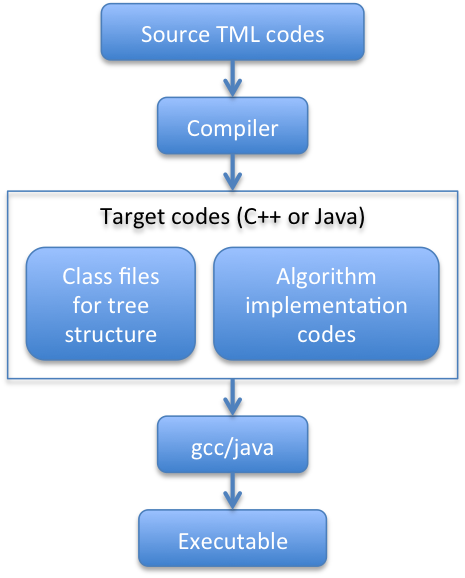
\includegraphics{Process.png}} \par}
\caption{TML Compiling Process}
\label{TCP}
\end{figure}

TML compiles the source codes and translate them into C++ or Java source code, which is then compiled by gcc or java into executable files. The C++ or Java codes in the middle of this process can also be used by programmers in other C++ or Java programs. Figure \ref{TCP} shows the compiling process of TML.

\section{Sample Code}

\begin{figure}[ht]
{\centering \resizebox*{60pt}{60pt}{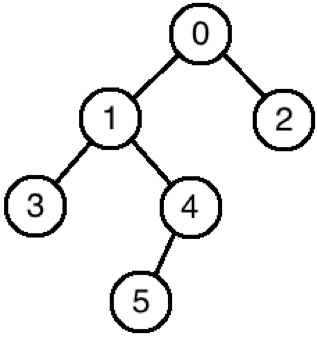
\includegraphics{tree.png}} \par}
\caption{Tree constrution in sample code}
\label{tree}
\end{figure}

\begin{lstlisting}
// Type definition of MyTree_t
// with Degree 2 and Storage of int.
Type MyTree_t <2, int>;

// Define six trees with initial values for root nodes.
MyTree_t a(0), b(1), c(2), d(3), e(4), f(5);
// Build a tree with six sub trees.
a -> ( b -> (d, e -> (f, _)), c);

// An example of inorder traversal.
forEach child in a by inorder do
{
	print(child);
}
\end{lstlisting}

\section{Syntax Draft}
\begin{description}
\item A.Basic\\
Every statement should end with semicolon.
\vspace{3mm}
Comments can be written as follows:
\begin{lstlisting}
//This is a single-line comment
/*
This is a multi-line comment
*/

\end{lstlisting}

\item B.Types\\
\begin{enumerate}
\item int\\
Type of integers.
\item float\\
Type of floating numbers.
\item char\\
Type of single characters.
\item string\\
Type of character sequences.
\item Tree\\
A tree structure containing a node and connections to its subtrees. Before using this type, a type definition should be in the following format to indicate the degrees, the name index of subtrees and the type of value of each nodes:

\begin{lstlisting}
Type MyTree\_t \textless 2[left, right], int\textgreater
\end{lstlisting}

\vspace{2mm}
This means MyTree\_t is a type of tree whose degree is at most 2 with the first subtree called left and second subtree called right. Also, each node of this tree contains an integer.

\vspace{2mm}
[left, right] part is optional. By default, the first subtree could be simply referred by number 0, and the second by number 1, and so on.

\vspace{2mm}
The keyword \textbf{\emph{Tree}} can be used directly as a type, which means no restrictions on degree and type of node values.

\end{enumerate}

\item C.Expressions\\
\begin{itemize}
\item Basic Operators:

\begin{table}[h]
\begin{tabular}{|l|l|}

\hline
expr1 + expr2 & Add two numbers, or concatenate two strings  \\
\hline
expr1 - expr2 & Subtraction  \\
\hline
expr1 * expr2 & Multiplication  \\
\hline
expr1 / expr2 &  \tabincell{l}{Division. If the value of expr1 and expr2 are both integers, the \\result is the integral part of the result. } \\
\hline
expr1 \% expr2 & The remainder part of the division \\
\hline
\textless, \textless=, ==, \textless\textgreater, \textgreater=, \textgreater &  Comparisons, returns 0 if false, 1 if true. \\
\hline
var = expr &  Assignments \\
\hline
\end{tabular}

\end{table}

\item Boolean Operators:
\begin{table}[h]
\begin{tabular}{|l|l|}

\hline
expr1 and expr2 & Logic and  \\
\hline
expr1 or expr2 & Logic or  \\
\hline
not expr & Logic not  \\
\hline

\end{tabular}

\end{table}

\item Tree Operators:
\begin{table}[h]
\begin{tabular}{|l|l|}

\hline
Tree[name]& \tabincell{l}{Get the subtree by its name index. The name index of subtrees is \\specified at tree type definition.} \\
\hline
Tree[integer] & \tabincell{l}{Get the subtree by its number, which is counted from the left. The\\ number of the first subtree is 0. } \\
\hline
Tree -\textgreater () & Assign all the subtrees. This assignment can be nested.  \\
\hline
@Tree &  Get the value of the root node \\
\hline
\^{}Tree & Get the parent of the subtree \\

\hline
\end{tabular}

\end{table}

\end{itemize}

\item D.Branches\\
There is only one kind of control statement-if:
\begin{lstlisting}
if expr then
{
	//Statements when expr is 1
}
else
{
	//Statements when expr is 0
}

\end{lstlisting}
\item E.Loops\\
There are three kinds of loops - for, while and forEach:
\begin{lstlisting}
for var = start_num to end_num by step do
{
	//Loop body
}
\end{lstlisting}
\begin{lstlisting}
while expr do
{
	//Loop when expr is 1
}
\end{lstlisting}
\begin{lstlisting}
forEach var in tree/string by function_iter do
{
	//each element in a tree or a string produces an iteration.
	//The elements will be iterated according to what is specified in function_iter
}

\end{lstlisting}
\item F.Functions\\

\begin{lstlisting}
return_type function_name (argument lists)
{
	//Statements
}
\end{lstlisting}
Each item in argument lists contains the type of the argument and its name, separated by commas.
\end{description}
\end{document} % DONE WITH DOCUMENT!


